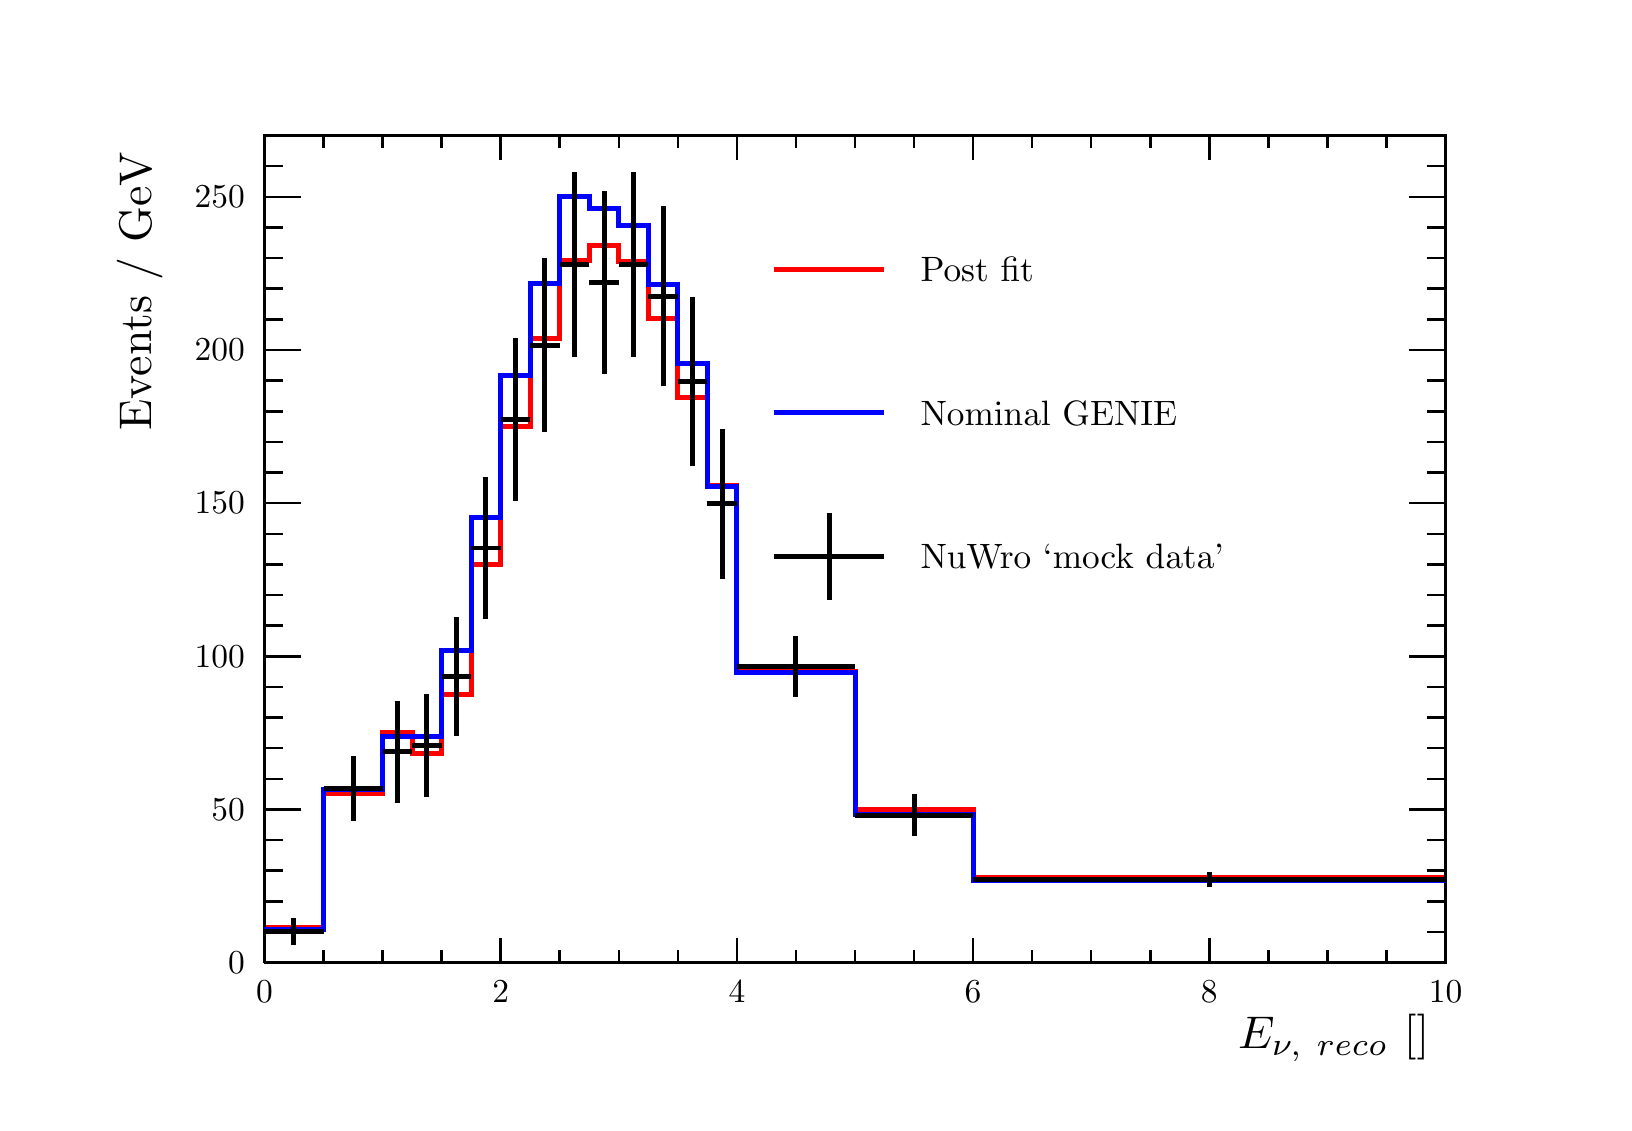
\begin{tikzpicture}
\pgfdeclareplotmark{cross} {
\pgfpathmoveto{\pgfpoint{-0.3\pgfplotmarksize}{\pgfplotmarksize}}
\pgfpathlineto{\pgfpoint{+0.3\pgfplotmarksize}{\pgfplotmarksize}}
\pgfpathlineto{\pgfpoint{+0.3\pgfplotmarksize}{0.3\pgfplotmarksize}}
\pgfpathlineto{\pgfpoint{+1\pgfplotmarksize}{0.3\pgfplotmarksize}}
\pgfpathlineto{\pgfpoint{+1\pgfplotmarksize}{-0.3\pgfplotmarksize}}
\pgfpathlineto{\pgfpoint{+0.3\pgfplotmarksize}{-0.3\pgfplotmarksize}}
\pgfpathlineto{\pgfpoint{+0.3\pgfplotmarksize}{-1.\pgfplotmarksize}}
\pgfpathlineto{\pgfpoint{-0.3\pgfplotmarksize}{-1.\pgfplotmarksize}}
\pgfpathlineto{\pgfpoint{-0.3\pgfplotmarksize}{-0.3\pgfplotmarksize}}
\pgfpathlineto{\pgfpoint{-1.\pgfplotmarksize}{-0.3\pgfplotmarksize}}
\pgfpathlineto{\pgfpoint{-1.\pgfplotmarksize}{0.3\pgfplotmarksize}}
\pgfpathlineto{\pgfpoint{-0.3\pgfplotmarksize}{0.3\pgfplotmarksize}}
\pgfpathclose
\pgfusepathqstroke
}
\pgfdeclareplotmark{cross*} {
\pgfpathmoveto{\pgfpoint{-0.3\pgfplotmarksize}{\pgfplotmarksize}}
\pgfpathlineto{\pgfpoint{+0.3\pgfplotmarksize}{\pgfplotmarksize}}
\pgfpathlineto{\pgfpoint{+0.3\pgfplotmarksize}{0.3\pgfplotmarksize}}
\pgfpathlineto{\pgfpoint{+1\pgfplotmarksize}{0.3\pgfplotmarksize}}
\pgfpathlineto{\pgfpoint{+1\pgfplotmarksize}{-0.3\pgfplotmarksize}}
\pgfpathlineto{\pgfpoint{+0.3\pgfplotmarksize}{-0.3\pgfplotmarksize}}
\pgfpathlineto{\pgfpoint{+0.3\pgfplotmarksize}{-1.\pgfplotmarksize}}
\pgfpathlineto{\pgfpoint{-0.3\pgfplotmarksize}{-1.\pgfplotmarksize}}
\pgfpathlineto{\pgfpoint{-0.3\pgfplotmarksize}{-0.3\pgfplotmarksize}}
\pgfpathlineto{\pgfpoint{-1.\pgfplotmarksize}{-0.3\pgfplotmarksize}}
\pgfpathlineto{\pgfpoint{-1.\pgfplotmarksize}{0.3\pgfplotmarksize}}
\pgfpathlineto{\pgfpoint{-0.3\pgfplotmarksize}{0.3\pgfplotmarksize}}
\pgfpathclose
\pgfusepathqfillstroke
}
\pgfdeclareplotmark{newstar} {
\pgfpathmoveto{\pgfqpoint{0pt}{\pgfplotmarksize}}
\pgfpathlineto{\pgfqpointpolar{44}{0.5\pgfplotmarksize}}
\pgfpathlineto{\pgfqpointpolar{18}{\pgfplotmarksize}}
\pgfpathlineto{\pgfqpointpolar{-20}{0.5\pgfplotmarksize}}
\pgfpathlineto{\pgfqpointpolar{-54}{\pgfplotmarksize}}
\pgfpathlineto{\pgfqpointpolar{-90}{0.5\pgfplotmarksize}}
\pgfpathlineto{\pgfqpointpolar{234}{\pgfplotmarksize}}
\pgfpathlineto{\pgfqpointpolar{198}{0.5\pgfplotmarksize}}
\pgfpathlineto{\pgfqpointpolar{162}{\pgfplotmarksize}}
\pgfpathlineto{\pgfqpointpolar{134}{0.5\pgfplotmarksize}}
\pgfpathclose
\pgfusepathqstroke
}
\pgfdeclareplotmark{newstar*} {
\pgfpathmoveto{\pgfqpoint{0pt}{\pgfplotmarksize}}
\pgfpathlineto{\pgfqpointpolar{44}{0.5\pgfplotmarksize}}
\pgfpathlineto{\pgfqpointpolar{18}{\pgfplotmarksize}}
\pgfpathlineto{\pgfqpointpolar{-20}{0.5\pgfplotmarksize}}
\pgfpathlineto{\pgfqpointpolar{-54}{\pgfplotmarksize}}
\pgfpathlineto{\pgfqpointpolar{-90}{0.5\pgfplotmarksize}}
\pgfpathlineto{\pgfqpointpolar{234}{\pgfplotmarksize}}
\pgfpathlineto{\pgfqpointpolar{198}{0.5\pgfplotmarksize}}
\pgfpathlineto{\pgfqpointpolar{162}{\pgfplotmarksize}}
\pgfpathlineto{\pgfqpointpolar{134}{0.5\pgfplotmarksize}}
\pgfpathclose
\pgfusepathqfillstroke
}
\definecolor{c}{rgb}{1,1,1};
\draw [color=c, fill=c] (0,0) rectangle (20,13.639);
\draw [color=c, fill=c] (3,1.77307) rectangle (18,12.2751);
\definecolor{c}{rgb}{0,0,0};
\draw [c,line width=0.9] (3,1.77307) -- (3,12.2751) -- (18,12.2751) -- (18,1.77307) -- (3,1.77307);
\definecolor{c}{rgb}{1,1,1};
\draw [color=c, fill=c] (3,1.77307) rectangle (18,12.2751);
\definecolor{c}{rgb}{0,0,0};
\draw [c,line width=0.9] (3,1.77307) -- (3,12.2751) -- (18,12.2751) -- (18,1.77307) -- (3,1.77307);
\definecolor{c}{rgb}{1,0,0};
\draw [c,line width=1.8] (3,2.22222) -- (3.75,2.22222) -- (3.75,3.92433) -- (4.5,3.92433) -- (4.5,4.70113) -- (4.875,4.70113) -- (4.875,4.42819) -- (5.25,4.42819) -- (5.25,5.17395) -- (5.625,5.17395) -- (5.625,6.82347) -- (6,6.82347) -- (6,8.57607)
 -- (6.375,8.57607) -- (6.375,9.70246) -- (6.75,9.70246) -- (6.75,10.6877) -- (7.125,10.6877) -- (7.125,10.8781) -- (7.5,10.8781) -- (7.5,10.6743) -- (7.875,10.6743) -- (7.875,9.95149) -- (8.25,9.95149) -- (8.25,8.94523) -- (8.625,8.94523) --
 (8.625,7.83099) -- (9,7.83099) -- (9,5.4682) -- (10.5,5.4682) -- (10.5,3.71794) -- (12,3.71794) -- (12,2.84826) -- (18,2.84826);
\definecolor{c}{rgb}{0,0,0};
\draw [c,line width=0.9] (3,1.77307) -- (18,1.77307);
\draw [c,line width=0.9] (3,2.07994) -- (3,1.77307);
\draw [c,line width=0.9] (3.75,1.9265) -- (3.75,1.77307);
\draw [c,line width=0.9] (4.5,1.9265) -- (4.5,1.77307);
\draw [c,line width=0.9] (5.25,1.9265) -- (5.25,1.77307);
\draw [c,line width=0.9] (6,2.07994) -- (6,1.77307);
\draw [c,line width=0.9] (6.75,1.9265) -- (6.75,1.77307);
\draw [c,line width=0.9] (7.5,1.9265) -- (7.5,1.77307);
\draw [c,line width=0.9] (8.25,1.9265) -- (8.25,1.77307);
\draw [c,line width=0.9] (9,2.07994) -- (9,1.77307);
\draw [c,line width=0.9] (9.75,1.9265) -- (9.75,1.77307);
\draw [c,line width=0.9] (10.5,1.9265) -- (10.5,1.77307);
\draw [c,line width=0.9] (11.25,1.9265) -- (11.25,1.77307);
\draw [c,line width=0.9] (12,2.07994) -- (12,1.77307);
\draw [c,line width=0.9] (12.75,1.9265) -- (12.75,1.77307);
\draw [c,line width=0.9] (13.5,1.9265) -- (13.5,1.77307);
\draw [c,line width=0.9] (14.25,1.9265) -- (14.25,1.77307);
\draw [c,line width=0.9] (15,2.07994) -- (15,1.77307);
\draw [c,line width=0.9] (15.75,1.9265) -- (15.75,1.77307);
\draw [c,line width=0.9] (16.5,1.9265) -- (16.5,1.77307);
\draw [c,line width=0.9] (17.25,1.9265) -- (17.25,1.77307);
\draw [c,line width=0.9] (18,2.07994) -- (18,1.77307);
\draw [anchor=base] (3,1.26842) node[scale=1.20912, color=c, rotate=0]{0};
\draw [anchor=base] (6,1.26842) node[scale=1.20912, color=c, rotate=0]{2};
\draw [anchor=base] (9,1.26842) node[scale=1.20912, color=c, rotate=0]{4};
\draw [anchor=base] (12,1.26842) node[scale=1.20912, color=c, rotate=0]{6};
\draw [anchor=base] (15,1.26842) node[scale=1.20912, color=c, rotate=0]{8};
\draw [anchor=base] (18,1.26842) node[scale=1.20912, color=c, rotate=0]{10};
\draw [anchor= east] (18,0.812882) node[scale=1.65459, color=c, rotate=0]{$E_{\nu,~\text{reco}}$ [\si{\GeV}]};
\draw [c,line width=0.9] (3,12.2751) -- (18,12.2751);
\draw [c,line width=0.9] (3,11.9682) -- (3,12.2751);
\draw [c,line width=0.9] (3.75,12.1216) -- (3.75,12.2751);
\draw [c,line width=0.9] (4.5,12.1216) -- (4.5,12.2751);
\draw [c,line width=0.9] (5.25,12.1216) -- (5.25,12.2751);
\draw [c,line width=0.9] (6,11.9682) -- (6,12.2751);
\draw [c,line width=0.9] (6.75,12.1216) -- (6.75,12.2751);
\draw [c,line width=0.9] (7.5,12.1216) -- (7.5,12.2751);
\draw [c,line width=0.9] (8.25,12.1216) -- (8.25,12.2751);
\draw [c,line width=0.9] (9,11.9682) -- (9,12.2751);
\draw [c,line width=0.9] (9.75,12.1216) -- (9.75,12.2751);
\draw [c,line width=0.9] (10.5,12.1216) -- (10.5,12.2751);
\draw [c,line width=0.9] (11.25,12.1216) -- (11.25,12.2751);
\draw [c,line width=0.9] (12,11.9682) -- (12,12.2751);
\draw [c,line width=0.9] (12.75,12.1216) -- (12.75,12.2751);
\draw [c,line width=0.9] (13.5,12.1216) -- (13.5,12.2751);
\draw [c,line width=0.9] (14.25,12.1216) -- (14.25,12.2751);
\draw [c,line width=0.9] (15,11.9682) -- (15,12.2751);
\draw [c,line width=0.9] (15.75,12.1216) -- (15.75,12.2751);
\draw [c,line width=0.9] (16.5,12.1216) -- (16.5,12.2751);
\draw [c,line width=0.9] (17.25,12.1216) -- (17.25,12.2751);
\draw [c,line width=0.9] (18,11.9682) -- (18,12.2751);
\draw [c,line width=0.9] (3,1.77307) -- (3,12.2751);
\draw [c,line width=0.9] (3.462,1.77307) -- (3,1.77307);
\draw [c,line width=0.9] (3.231,2.16203) -- (3,2.16203);
\draw [c,line width=0.9] (3.231,2.55099) -- (3,2.55099);
\draw [c,line width=0.9] (3.231,2.93996) -- (3,2.93996);
\draw [c,line width=0.9] (3.231,3.32892) -- (3,3.32892);
\draw [c,line width=0.9] (3.462,3.71788) -- (3,3.71788);
\draw [c,line width=0.9] (3.231,4.10684) -- (3,4.10684);
\draw [c,line width=0.9] (3.231,4.49581) -- (3,4.49581);
\draw [c,line width=0.9] (3.231,4.88477) -- (3,4.88477);
\draw [c,line width=0.9] (3.231,5.27373) -- (3,5.27373);
\draw [c,line width=0.9] (3.462,5.6627) -- (3,5.6627);
\draw [c,line width=0.9] (3.231,6.05166) -- (3,6.05166);
\draw [c,line width=0.9] (3.231,6.44062) -- (3,6.44062);
\draw [c,line width=0.9] (3.231,6.82959) -- (3,6.82959);
\draw [c,line width=0.9] (3.231,7.21855) -- (3,7.21855);
\draw [c,line width=0.9] (3.462,7.60751) -- (3,7.60751);
\draw [c,line width=0.9] (3.231,7.99648) -- (3,7.99648);
\draw [c,line width=0.9] (3.231,8.38544) -- (3,8.38544);
\draw [c,line width=0.9] (3.231,8.7744) -- (3,8.7744);
\draw [c,line width=0.9] (3.231,9.16337) -- (3,9.16337);
\draw [c,line width=0.9] (3.462,9.55233) -- (3,9.55233);
\draw [c,line width=0.9] (3.231,9.94129) -- (3,9.94129);
\draw [c,line width=0.9] (3.231,10.3303) -- (3,10.3303);
\draw [c,line width=0.9] (3.231,10.7192) -- (3,10.7192);
\draw [c,line width=0.9] (3.231,11.1082) -- (3,11.1082);
\draw [c,line width=0.9] (3.462,11.4971) -- (3,11.4971);
\draw [c,line width=0.9] (3.462,11.4971) -- (3,11.4971);
\draw [c,line width=0.9] (3.231,11.8861) -- (3,11.8861);
\draw [c,line width=0.9] (3.231,12.2751) -- (3,12.2751);
\draw [anchor= east] (2.9,1.77307) node[scale=1.20912, color=c, rotate=0]{0};
\draw [anchor= east] (2.9,3.71788) node[scale=1.20912, color=c, rotate=0]{50};
\draw [anchor= east] (2.9,5.6627) node[scale=1.20912, color=c, rotate=0]{100};
\draw [anchor= east] (2.9,7.60751) node[scale=1.20912, color=c, rotate=0]{150};
\draw [anchor= east] (2.9,9.55233) node[scale=1.20912, color=c, rotate=0]{200};
\draw [anchor= east] (2.9,11.4971) node[scale=1.20912, color=c, rotate=0]{250};
\draw [anchor= east] (1.416,12.2751) node[scale=1.65459, color=c, rotate=90]{Events / GeV};
\draw [c,line width=0.9] (18,1.77307) -- (18,12.2751);
\draw [c,line width=0.9] (17.538,1.77307) -- (18,1.77307);
\draw [c,line width=0.9] (17.769,2.16203) -- (18,2.16203);
\draw [c,line width=0.9] (17.769,2.55099) -- (18,2.55099);
\draw [c,line width=0.9] (17.769,2.93996) -- (18,2.93996);
\draw [c,line width=0.9] (17.769,3.32892) -- (18,3.32892);
\draw [c,line width=0.9] (17.538,3.71788) -- (18,3.71788);
\draw [c,line width=0.9] (17.769,4.10684) -- (18,4.10684);
\draw [c,line width=0.9] (17.769,4.49581) -- (18,4.49581);
\draw [c,line width=0.9] (17.769,4.88477) -- (18,4.88477);
\draw [c,line width=0.9] (17.769,5.27373) -- (18,5.27373);
\draw [c,line width=0.9] (17.538,5.6627) -- (18,5.6627);
\draw [c,line width=0.9] (17.769,6.05166) -- (18,6.05166);
\draw [c,line width=0.9] (17.769,6.44062) -- (18,6.44062);
\draw [c,line width=0.9] (17.769,6.82959) -- (18,6.82959);
\draw [c,line width=0.9] (17.769,7.21855) -- (18,7.21855);
\draw [c,line width=0.9] (17.538,7.60751) -- (18,7.60751);
\draw [c,line width=0.9] (17.769,7.99648) -- (18,7.99648);
\draw [c,line width=0.9] (17.769,8.38544) -- (18,8.38544);
\draw [c,line width=0.9] (17.769,8.7744) -- (18,8.7744);
\draw [c,line width=0.9] (17.769,9.16337) -- (18,9.16337);
\draw [c,line width=0.9] (17.538,9.55233) -- (18,9.55233);
\draw [c,line width=0.9] (17.769,9.94129) -- (18,9.94129);
\draw [c,line width=0.9] (17.769,10.3303) -- (18,10.3303);
\draw [c,line width=0.9] (17.769,10.7192) -- (18,10.7192);
\draw [c,line width=0.9] (17.769,11.1082) -- (18,11.1082);
\draw [c,line width=0.9] (17.538,11.4971) -- (18,11.4971);
\draw [c,line width=0.9] (17.538,11.4971) -- (18,11.4971);
\draw [c,line width=0.9] (17.769,11.8861) -- (18,11.8861);
\draw [c,line width=0.9] (17.769,12.2751) -- (18,12.2751);
\definecolor{c}{rgb}{0,0,1};
\draw [c,line width=1.8] (3,2.19439) -- (3.75,2.19439) -- (3.75,3.97436) -- (4.5,3.97436) -- (4.5,4.64849) -- (4.875,4.64849) -- (4.875,4.63969) -- (5.25,4.63969) -- (5.25,5.73757) -- (5.625,5.73757) -- (5.625,7.42329) -- (6,7.42329) -- (6,9.2341) --
 (6.375,9.2341) -- (6.375,10.4005) -- (6.75,10.4005) -- (6.75,11.5064) -- (7.125,11.5064) -- (7.125,11.3462) -- (7.5,11.3462) -- (7.5,11.1353) -- (7.875,11.1353) -- (7.875,10.3888) -- (8.25,10.3888) -- (8.25,9.38121) -- (8.625,9.38121) --
 (8.625,7.82402) -- (9,7.82402) -- (9,5.45115) -- (10.5,5.45115) -- (10.5,3.65539) -- (12,3.65539) -- (12,2.81291) -- (18,2.81291);
\definecolor{c}{rgb}{0,0,0};
\draw [c,line width=1.8] (3.375,1.99374) -- (3.375,2.16932);
\draw [c,line width=1.8] (3.375,2.16932) -- (3.375,2.34489);
\draw [c,line width=1.8] (3,2.16932) -- (3.375,2.16932);
\draw [c,line width=1.8] (3.375,2.16932) -- (3.75,2.16932);
\foreach \P in {(3.375,2.16932)}{\draw[mark options={color=c,fill=c},mark size=2.402402pt, line width=0.000000pt, mark=*,mark size=1pt] plot coordinates {\P};}
\draw [c,line width=1.8] (4.125,3.56784) -- (4.125,3.98242);
\draw [c,line width=1.8] (4.125,3.98242) -- (4.125,4.39699);
\draw [c,line width=1.8] (3.75,3.98242) -- (4.125,3.98242);
\draw [c,line width=1.8] (4.125,3.98242) -- (4.5,3.98242);
\foreach \P in {(4.125,3.98242)}{\draw[mark options={color=c,fill=c},mark size=2.402402pt, line width=0.000000pt, mark=*,mark size=1pt] plot coordinates {\P};}
\draw [c,line width=1.8] (4.6875,3.80466) -- (4.6875,4.45002);
\draw [c,line width=1.8] (4.6875,4.45002) -- (4.6875,5.09539);
\draw [c,line width=1.8] (4.5,4.45002) -- (4.6875,4.45002);
\draw [c,line width=1.8] (4.6875,4.45002) -- (4.875,4.45002);
\foreach \P in {(4.6875,4.45002)}{\draw[mark options={color=c,fill=c},mark size=2.402402pt, line width=0.000000pt, mark=*,mark size=1pt] plot coordinates {\P};}
\draw [c,line width=1.8] (5.0625,3.87508) -- (5.0625,4.53001);
\draw [c,line width=1.8] (5.0625,4.53001) -- (5.0625,5.18495);
\draw [c,line width=1.8] (4.875,4.53001) -- (5.0625,4.53001);
\draw [c,line width=1.8] (5.0625,4.53001) -- (5.25,4.53001);
\foreach \P in {(5.0625,4.53001)}{\draw[mark options={color=c,fill=c},mark size=2.402402pt, line width=0.000000pt, mark=*,mark size=1pt] plot coordinates {\P};}
\draw [c,line width=1.8] (5.4375,4.65588) -- (5.4375,5.4079);
\draw [c,line width=1.8] (5.4375,5.4079) -- (5.4375,6.15991);
\draw [c,line width=1.8] (5.25,5.4079) -- (5.4375,5.4079);
\draw [c,line width=1.8] (5.4375,5.4079) -- (5.625,5.4079);
\foreach \P in {(5.4375,5.4079)}{\draw[mark options={color=c,fill=c},mark size=2.402402pt, line width=0.000000pt, mark=*,mark size=1pt] plot coordinates {\P};}
\draw [c,line width=1.8] (5.8125,6.13281) -- (5.8125,7.03787);
\draw [c,line width=1.8] (5.8125,7.03787) -- (5.8125,7.94292);
\draw [c,line width=1.8] (5.625,7.03787) -- (5.8125,7.03787);
\draw [c,line width=1.8] (5.8125,7.03787) -- (6,7.03787);
\foreach \P in {(5.8125,7.03787)}{\draw[mark options={color=c,fill=c},mark size=2.402402pt, line width=0.000000pt, mark=*,mark size=1pt] plot coordinates {\P};}
\draw [c,line width=1.8] (6.1875,7.63827) -- (6.1875,8.67449);
\draw [c,line width=1.8] (6.1875,8.67449) -- (6.1875,9.71072);
\draw [c,line width=1.8] (6,8.67449) -- (6.1875,8.67449);
\draw [c,line width=1.8] (6.1875,8.67449) -- (6.375,8.67449);
\foreach \P in {(6.1875,8.67449)}{\draw[mark options={color=c,fill=c},mark size=2.402402pt, line width=0.000000pt, mark=*,mark size=1pt] plot coordinates {\P};}
\draw [c,line width=1.8] (6.5625,8.50959) -- (6.5625,9.6141);
\draw [c,line width=1.8] (6.5625,9.6141) -- (6.5625,10.7186);
\draw [c,line width=1.8] (6.375,9.6141) -- (6.5625,9.6141);
\draw [c,line width=1.8] (6.5625,9.6141) -- (6.75,9.6141);
\foreach \P in {(6.5625,9.6141)}{\draw[mark options={color=c,fill=c},mark size=2.402402pt, line width=0.000000pt, mark=*,mark size=1pt] plot coordinates {\P};}
\draw [c,line width=1.8] (6.9375,9.46363) -- (6.9375,10.638);
\draw [c,line width=1.8] (6.9375,10.638) -- (6.9375,11.8125);
\draw [c,line width=1.8] (6.75,10.638) -- (6.9375,10.638);
\draw [c,line width=1.8] (6.9375,10.638) -- (7.125,10.638);
\foreach \P in {(6.9375,10.638)}{\draw[mark options={color=c,fill=c},mark size=2.402402pt, line width=0.000000pt, mark=*,mark size=1pt] plot coordinates {\P};}
\draw [c,line width=1.8] (7.3125,9.25262) -- (7.3125,10.412);
\draw [c,line width=1.8] (7.3125,10.412) -- (7.3125,11.5713);
\draw [c,line width=1.8] (7.125,10.412) -- (7.3125,10.412);
\draw [c,line width=1.8] (7.3125,10.412) -- (7.5,10.412);
\foreach \P in {(7.3125,10.412)}{\draw[mark options={color=c,fill=c},mark size=2.402402pt, line width=0.000000pt, mark=*,mark size=1pt] plot coordinates {\P};}
\draw [c,line width=1.8] (7.6875,9.46133) -- (7.6875,10.6356);
\draw [c,line width=1.8] (7.6875,10.6356) -- (7.6875,11.8098);
\draw [c,line width=1.8] (7.5,10.6356) -- (7.6875,10.6356);
\draw [c,line width=1.8] (7.6875,10.6356) -- (7.875,10.6356);
\foreach \P in {(7.6875,10.6356)}{\draw[mark options={color=c,fill=c},mark size=2.402402pt, line width=0.000000pt, mark=*,mark size=1pt] plot coordinates {\P};}
\draw [c,line width=1.8] (8.0625,9.08929) -- (8.0625,10.2368);
\draw [c,line width=1.8] (8.0625,10.2368) -- (8.0625,11.3844);
\draw [c,line width=1.8] (7.875,10.2368) -- (8.0625,10.2368);
\draw [c,line width=1.8] (8.0625,10.2368) -- (8.25,10.2368);
\foreach \P in {(8.0625,10.2368)}{\draw[mark options={color=c,fill=c},mark size=2.402402pt, line width=0.000000pt, mark=*,mark size=1pt] plot coordinates {\P};}
\draw [c,line width=1.8] (8.4375,8.07825) -- (8.4375,9.14954);
\draw [c,line width=1.8] (8.4375,9.14954) -- (8.4375,10.2208);
\draw [c,line width=1.8] (8.25,9.14954) -- (8.4375,9.14954);
\draw [c,line width=1.8] (8.4375,9.14954) -- (8.625,9.14954);
\foreach \P in {(8.4375,9.14954)}{\draw[mark options={color=c,fill=c},mark size=2.402402pt, line width=0.000000pt, mark=*,mark size=1pt] plot coordinates {\P};}
\draw [c,line width=1.8] (8.8125,6.64985) -- (8.8125,7.60218);
\draw [c,line width=1.8] (8.8125,7.60218) -- (8.8125,8.5545);
\draw [c,line width=1.8] (8.625,7.60218) -- (8.8125,7.60218);
\draw [c,line width=1.8] (8.8125,7.60218) -- (9,7.60218);
\foreach \P in {(8.8125,7.60218)}{\draw[mark options={color=c,fill=c},mark size=2.402402pt, line width=0.000000pt, mark=*,mark size=1pt] plot coordinates {\P};}
\draw [c,line width=1.8] (9.75,5.14946) -- (9.75,5.53182);
\draw [c,line width=1.8] (9.75,5.53182) -- (9.75,5.91419);
\draw [c,line width=1.8] (9,5.53182) -- (9.75,5.53182);
\draw [c,line width=1.8] (9.75,5.53182) -- (10.5,5.53182);
\foreach \P in {(9.75,5.53182)}{\draw[mark options={color=c,fill=c},mark size=2.402402pt, line width=0.000000pt, mark=*,mark size=1pt] plot coordinates {\P};}
\draw [c,line width=1.8] (11.25,3.37557) -- (11.25,3.64544);
\draw [c,line width=1.8] (11.25,3.64544) -- (11.25,3.9153);
\draw [c,line width=1.8] (10.5,3.64544) -- (11.25,3.64544);
\draw [c,line width=1.8] (11.25,3.64544) -- (12,3.64544);
\foreach \P in {(11.25,3.64544)}{\draw[mark options={color=c,fill=c},mark size=2.402402pt, line width=0.000000pt, mark=*,mark size=1pt] plot coordinates {\P};}
\draw [c,line width=1.8] (15,2.72638) -- (15,2.82765);
\draw [c,line width=1.8] (15,2.82765) -- (15,2.92891);
\draw [c,line width=1.8] (12,2.82765) -- (15,2.82765);
\draw [c,line width=1.8] (15,2.82765) -- (18,2.82765);
\foreach \P in {(15,2.82765)}{\draw[mark options={color=c,fill=c},mark size=2.402402pt, line width=0.000000pt, mark=*,mark size=1pt] plot coordinates {\P};}
\definecolor{c}{rgb}{1,1,1};
\draw [color=c, fill=c] (2,12.8206) rectangle (18,13.5708);
\definecolor{c}{rgb}{0,0,0};
%\draw (10,13.1957) node[scale=1.40004, color=c, rotate=0]{$\nu_{e} RHC postfit: \delta = 1.57, \chi^{2} = 51.36$};
\definecolor{c}{rgb}{1,1,1};
\draw [color=c, fill=c] (9.16905,6.01719) rectangle (17.192,11.49);
\definecolor{c}{rgb}{0,0,0};
\draw [anchor= west] (11.1748,10.5778) node[scale=1.27276, color=c, rotate=0]{Post fit};
\definecolor{c}{rgb}{1,0,0};
\draw [c,line width=1.8] (9.46991,10.5778) -- (10.8739,10.5778);
\definecolor{c}{rgb}{0,0,0};
\draw [anchor= west] (11.1748,8.75358) node[scale=1.27276, color=c, rotate=0]{Nominal GENIE};
\definecolor{c}{rgb}{0,0,1};
\draw [c,line width=1.8] (9.46991,8.75358) -- (10.8739,8.75358);
\definecolor{c}{rgb}{0,0,0};
\draw [anchor= west] (11.1748,6.92932) node[scale=1.27276, color=c, rotate=0]{NuWro `mock data'};
\draw [c,line width=1.8] (9.46991,6.92932) -- (10.8739,6.92932);
\draw [c,line width=1.8] (10.1719,6.38204) -- (10.1719,7.4766);
\end{tikzpicture}
